% !TeX spellcheck = en_US

\chapter{Results}

In this project, we have made nine experiments by varying the $K$-fold value in cross-validation: 2, 3, 5, 10, 20, 50, 150, 300, 750. The program has been written with the purpose to print all the results in \texttt{json} format, for an easier data analysis through python. In all of the experiments, both AdaBoost and Bagging have been trained over the same data-set with the same hyper-parameter $T$ varying at each cycle.\\
\begin{figure}[htpb]
	\centering
	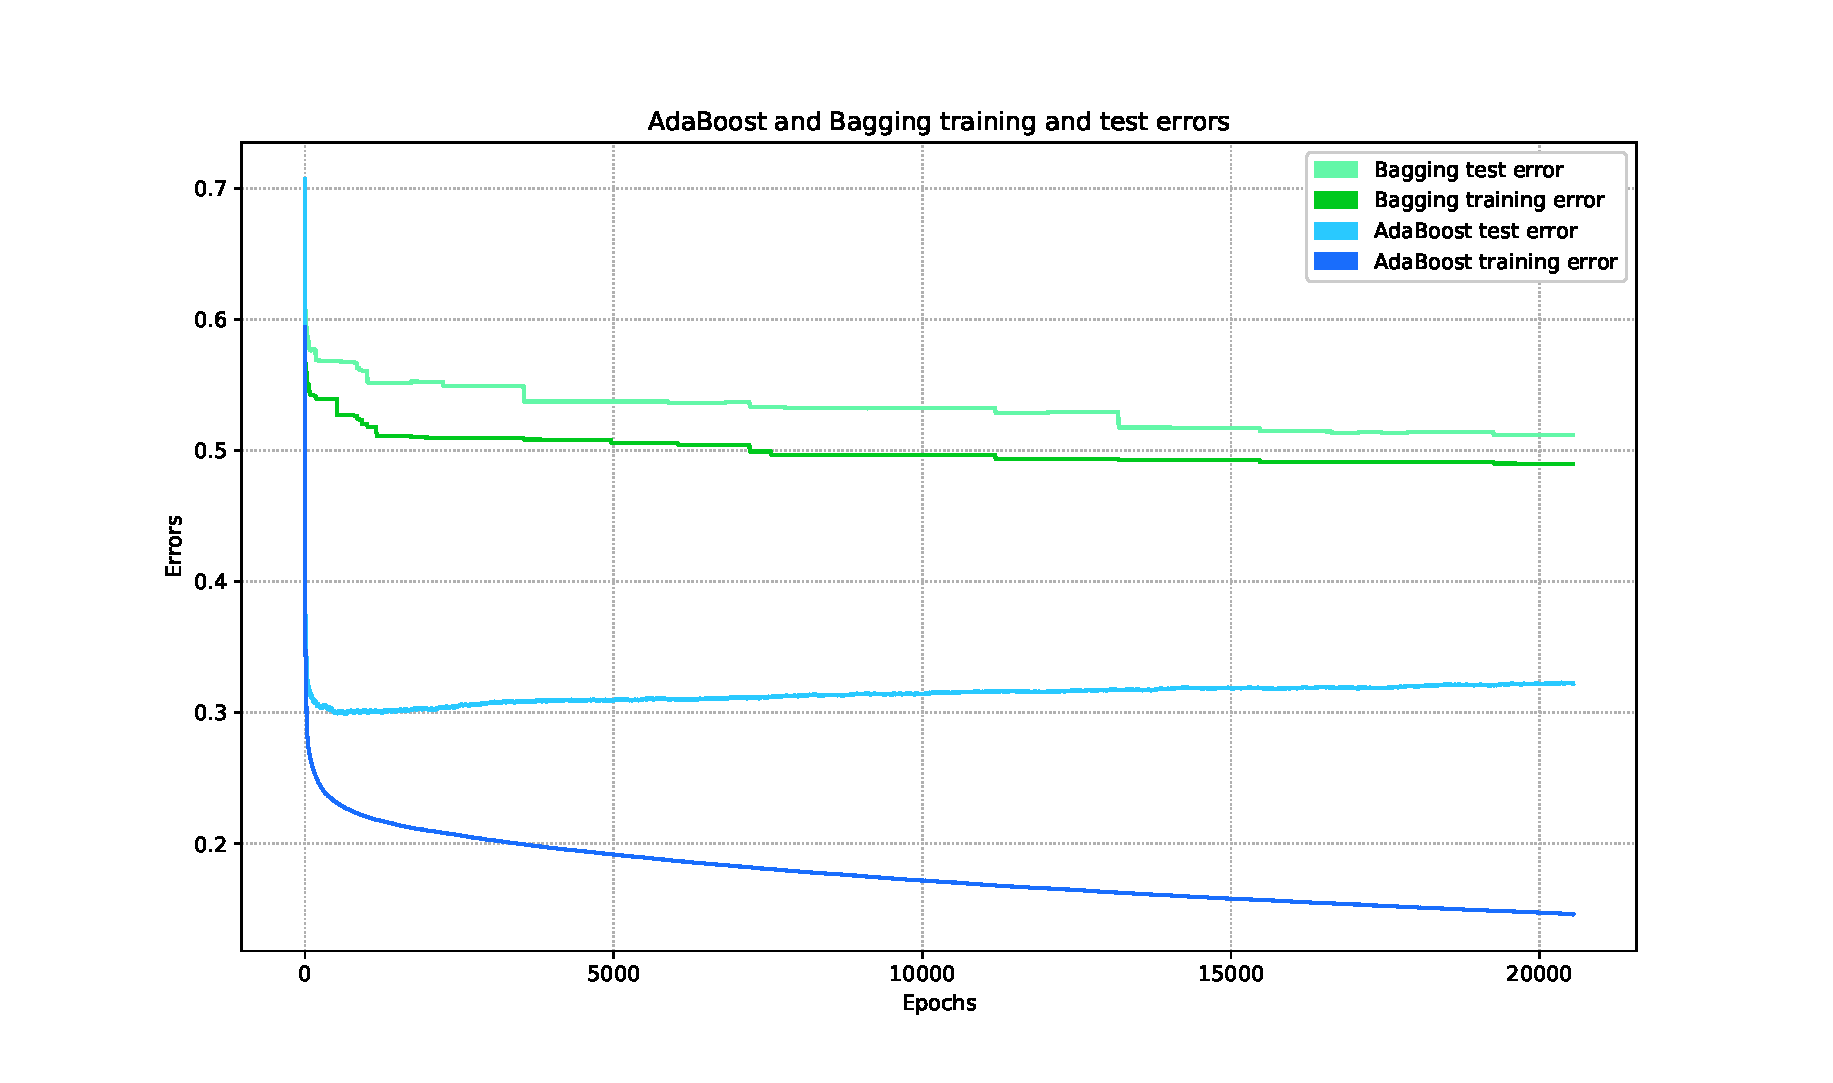
\includegraphics[scale=0.35]{figs/report_k20.eps}
	\label{fig:k20}
	\caption{A train for both AdaBoost and Bagging for circa 20000 epochs}
\end{figure}
As you can see in \figurename~\ref{fig:k20}, AdaBoost is way better than Bagging and it's already possible to catch the best value for $T$, which in that figure seems to be around the first thousands epochs. 
